O grupo 1 da disciplina de Projeto Integrador 1 do segundo semestre de 2015 deverá desenvolver um projeto de balão cativo para monitoramento do estacionamento e das fronteiras do campus da FGA, cujo objetivo é manter um maior controle da movimentação de carros e pessoas nas áreas de alcance do balão, devido os problemas de furtos avaliados anteriormente e, também, devido a possíveis invasões de área.

O estacionamento possui área de 16100 $m^2$, com perímetro de 1215 m. Contudo, a área é extensa e existem locais de estacionamento isolados [figura \ref{img:fga2}].

\begin{figure}[H]
  \centering
  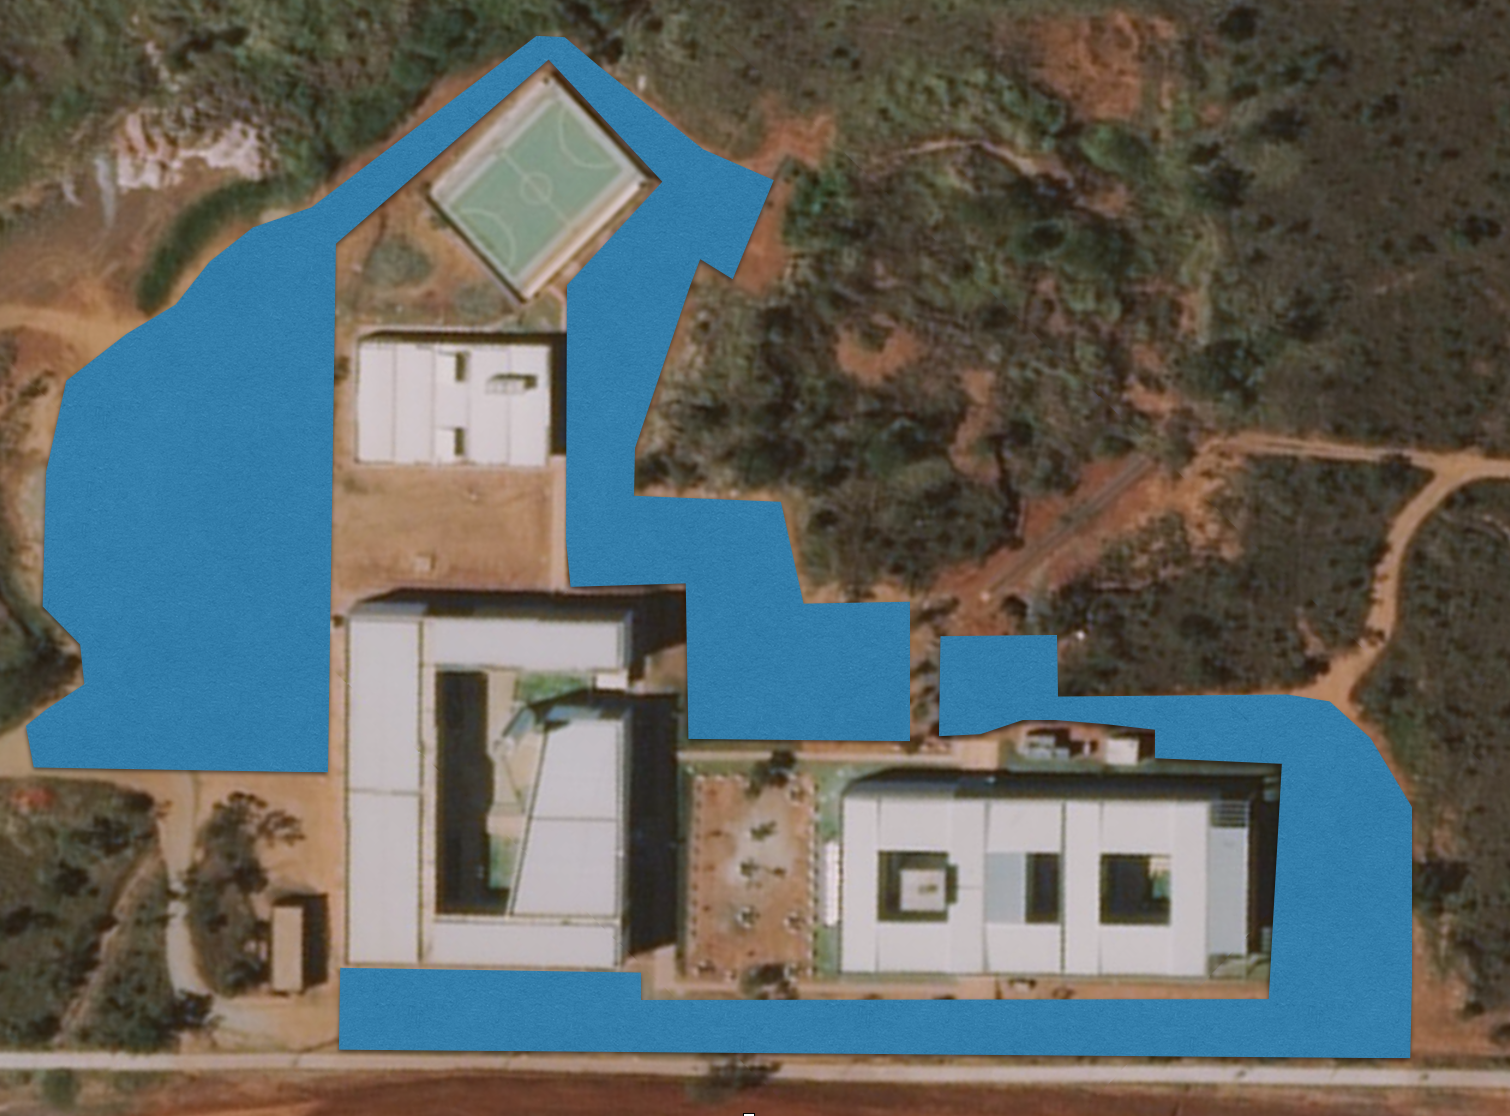
\includegraphics[width=0.87\textwidth]{figuras/fga2}
  \caption{Vista aérea do Campus FGA: áreas de estacionamento do campus.}
  \label{img:fga2}
\end{figure}

Dessa forma, devido à impossibilidade de localizar apenas um balão que possa monitorar todas as áreas de estacionamento, três balões cativos serão posicionados estrategicamente para que o objetivo seja cumprido [figura \ref{img:fga3}].

\begin{figure}[H]
  \centering
  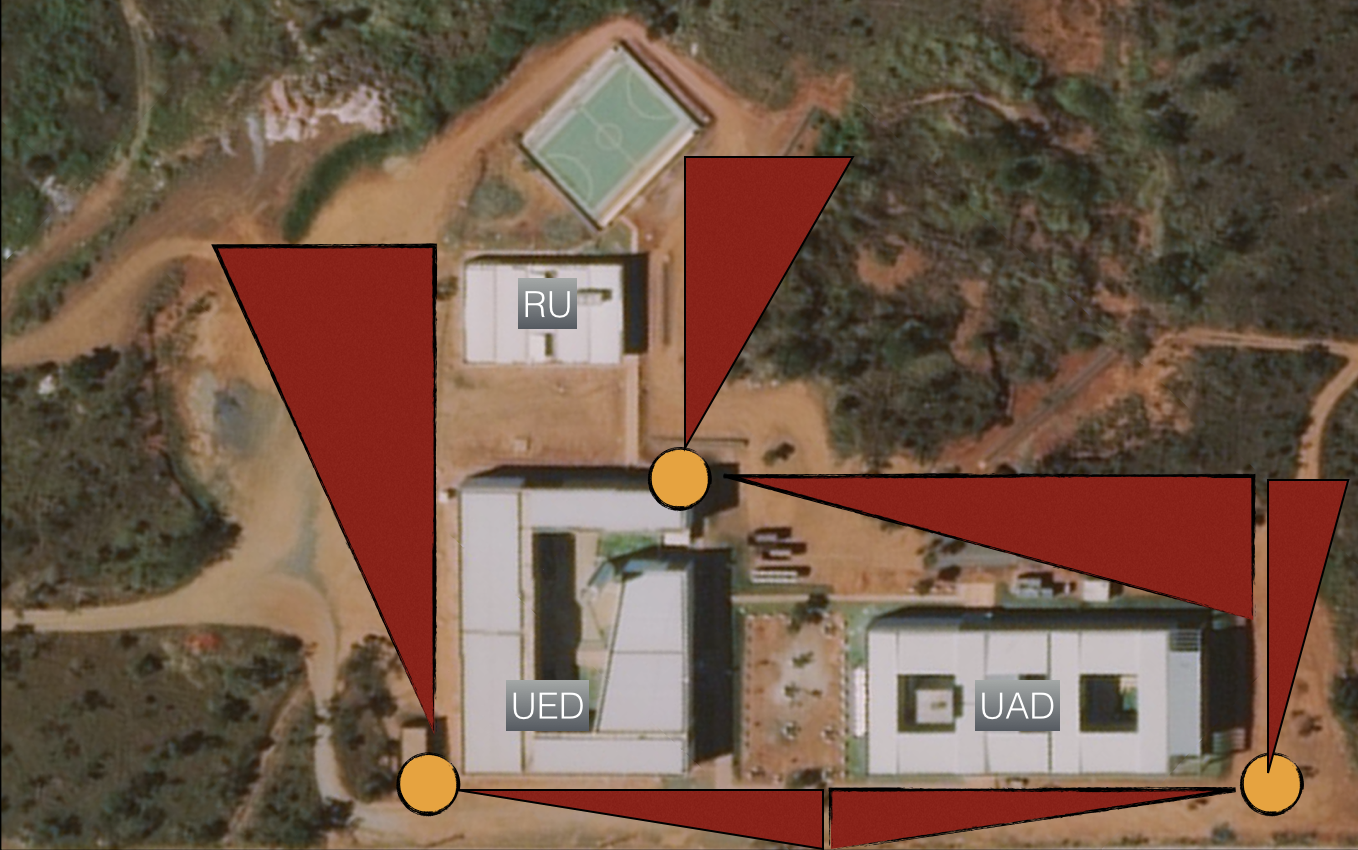
\includegraphics[width=0.87\textwidth]{figuras/fga3}
  \caption{Vista aérea do Campus FGA: áreas de alcance de monitoramento.}
  \label{img:fga3}
\end{figure}

\section{Estrutura e Funcionamento}
  A estrutura do balão será dividida em três partes principais: a bexiga, local onde será armazenado o gás; payload, que será o local de armazenamento dos equipamentos eletrônicos; elevador, que consite o cabo preso à payload do balão e também o sistema eletromecânico em solo que libera o fio (elevando o balão) ou retrai o fio (desce o balão).

  \subsection{Payload}
    A estrutura da payload foi inspirada em um padrão de nanosatélites 9U, figura \ref{img:payload}, porém com adaptações. A estrutura de um CubeSat 1U possui as dimensões deste são de um cubo 10 x 10 x 10 cm, ou seja, o termo 1U diz respeito as dimensões do sistema. Dessa forma um 9U significa que suas dimensões são 30 x 30 x 10 cm, e colocando de outra forma, é equivalente à três nanosatélites 3U em conjunto. A parte superior será acoplada à bexiga, enquanto que a inferior, ao cabo.

    \begin{figure}[H]
      \centering
      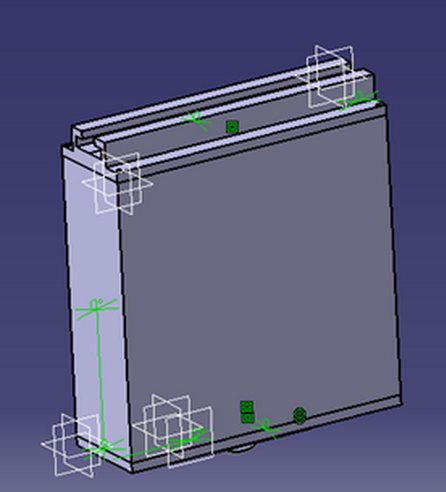
\includegraphics[width=0.5\textwidth]{figuras/payload}
      \caption{Representação da estrutura da payload. }
      \label{img:payload}
    \end{figure}

  \subsection{Balão}
    Segundo Yajima, existem três tipos de sistemas de balões que são utilizados: balão zero pressão, balão super-pressão e uma combinação entre os dois sistemas. O sistema mais adequado à aplicação proposta mostrou-se o balão zero pressão.Existem vários modelos de balão: esférico, cilíndrico, tetraédrico e formato natural. O modelo utilizado será o modelo de balão esférico, pois esse modelo é o que apresenta menos complicações nos cálculos de dimensionamento de volume, empuxo, gás e etc.

  \subsection{Gás}
    O gás que será utilizado no balão será o Hélio, este gás possui algumas desvantagens em relação ao gás Hidrogênio[2], que é mais leve, porém por ser um gás inerte o Hélio é a principal opção  de uso[3]. Ficou decidido que a massa  máxima  da payload será de 20 kg.

  \subsection{Material}
    O material usado para a confecção da bexiga será a Aramida (Kevlar), pois  esse material apresenta propriedades mecânicas interessantes, como elevada tenacidade, baixo alongamento e resistência ao calor[10],  além de ser considerado um material leve[8]. Com esses dados em mãos foi possível calcular o raio mínimo que o balão deveria ter, o valor foi de 2 metros. Para uma margem de segurança será adotado um valor de raio do balão entre 2 metros e 2,5 metros. As forças de empuxo e peso do balão variam de acordo com o raio. O empuxo com o raio igual a 2 metros é de cerca de 403N, com o raio igual a 2,5 metros o empuxo é de 786N, será avaliado o material utilizado na ancoragem do balão,  e dependendo da resistencia à tração desse material será adotado um raio fixo para o balão.

  \subsection{Funcionamento}
    O horário de funcionamento do balão será das 6h às 21h, o sistema ficará a uma altura entre 30 metros e 50 metros para uma melhor visualização do movimento do estacionamento.

    O estudo das condições ambientais e o dimensionamento dessas variáveis são fundamentais para a estabilidade do balão. A força de arrasto no balão devido a um vento de 12m/s, na pior das hióteses, seria na ordem de 3,8kN.

\section{Alimentação}

  \subsection{Tipos de Alimentação}
  Para a alimentação do aeróstato de monitoramento do estacionamento da Faculdade do Gama foram consideradas três possibilidades: energia solar, eólica e a cabo.  Contudo, é preciso analisar, de maneira objetiva e realista, a opção que melhor  atende às demandas de seu funcionamento, ao ambiente no qual o balão estará localizado e à viabilidade econômica de sua manutenção.

  Dessa forma, necessita-se de uma avaliação concisa das três opções disponíveis, abrangendo sua eficiência, operacionabilidade, custos e manutenção, respectivamente.

    \subsubsection{Energia Solar}
    Painéis solares fotovoltáicos, são dispositivos usualmente utilizados para conversão de energia proveniente do sol, em energia elétrica. Estruturalmente, painéis solares são compostos por células solares, capazes de criar uma DDP (Diferença de Potencial) através do fluxo de corrente elétrica.

      \paragraph{Eficiência}
      Eficiência é atingir o resultado com o mínimo de perdas de recurso, e quando falamos em uma placa fotovoltáica, falamos na quantidade de energia recebida, convertida em energia elétrica disponível para utilização. Em um painel solar, quanto maior a produção energética por metro quadrado de placa, melhor a eficiência do sistema. Atualmente, a média de valores referente à eficiência dos painéis solares comerciais fica entre 14\% e 21\%.

      \paragraph{Operacionabilidade}
      Inicialmente, devemos analisar o consumo energético,em kWh, que será demandado pelo aeróstato cativo, com base nisso, é feito o dimensionamento do sistema de geração.

      Após a estimativa de consumo, o próximo passo é a instalação dos painéis solares, levando em conta o direcionamento, inclinação, posição geográfica e incidência solar mensal. Para isso, existem softwares os quais auxiliam no processo de apontamento, aumentando a eficiência do sistema.

      Finalizando todas as etapas de dimensionamento, instalação, apontamento e análise dos dados de geração, o processo pode ser considerado simples, e de baixa complexidade de opreação para pequenos sistemas.

      \paragraph{Custos}
      Os custos iniciais de implantação de um sistema solar no Brasil, ainda é muito caro, devido a maior parte dos componentes serem importados e taxados com impostos e a opção começa a se tornar pouco atraente quando levamos em conta sua eficiência e comparamos com outros sistemas de geração

      \paragraph{Manutenção}
      A manutenção dos painéis solares é simples, de baixo custo, e o processo não precisa de mão de obra extremamente especializada. De forma simplificada, a manutenção do painel consiste na limpeza das superfícies, uma verificação do cabeamento, e correções no apontamento de tempos em tempos.

    \subsubsection{Energia Eólica}
    Devido a sua característica inesgotável e não poluidora, sendo, portanto, uma fonte de energia renovável, a energia eólica vem tomando espaço no estudo sobre aerogeradores \cite{rocha2010}. Segundo \cite{Evans20091082}, é um sistema que com menor emissão de CO2, com apenas 25 g/kW h CO2-e.

      \paragraph{Eficiência}
      Segundo \cite{Evans20091082}, a eficiência energética da energia eólica está entre 24-54%.

      \paragraph{Operacionabilidade}
      O modelo de aerogerador poderá apresentar eixo horizontal, com rotor em forma de balão de hélio, com transmissão de força para baixo pelo auxílio de cabos, bem como é apresentado no projeto da empresa Magenn Air Rotor System (MARS) \cite{texeira2012}.

      Podendo as turbinas sofrerem intermitência, \cite{edmondes2007}. propõe uma capacidade distribuída sobre uma ampla área, aliviando as flutuações. As turbinas não podem operar quando a velocidade do vento é muito alta (>25 m/s), pelo fato de que danos na turbina podem ocorrer e estas não poderão funcionar quando a velocidade do vento estiver muito baixa (< 3 m/s) (WEC, 2007).

      \paragraph{Custos}
      Mesmo se tratando de uma fonte de energia limpa, os custos de instalação de tecnologias para geração de energia elétrica são muito altos. Principalmente no Brasil, tendo em vista que o custo elevado pode se dar aos custos logísticos de implantação do projeto, como o número restrito de ofertantes nacionais também associado às restrições de importação de aerogeradores.

      A oferta de turbinas eólicas no Brasil se restringe apenas a duas firmas que possuem suas vantagens, entre elas: imposto de 14\% sobre a importação de aerogeradores, sendo que apenas aqueles que possuem potência superior a 1,5 MW que poderão ser importados e o BNDES só concede financiamento aos fabricantes nacionais.

      O custo de manutenção para turbinas no inicio de sua vida útil normalmente é mais baixo quando comparado com o custo para turbinas que tenham maior tempo de funcionamento. Para máquinas novas, é estimado um custo anual de 1,5 a 2\% do investimento, enquanto para turbinas com maior tempo de funcionamento o custo do investimento sai em torno de 3\% ao ano.

      \paragraph{Manutenção}
      Os sistemas eólicos necessitam de pouca manutenção. A vida útil de suas turbinas eólicas é de 15 anos, e os dispositivos eletrônicos, como inversor e controlador de carga, são avaliados em 10 anos. Já os sistemas eólicos isolados com o armazenamento de energia em baterias, as quais são consideradas o ponto crítico do sistema, que quando bem projetado poderá ter uma vida útil de 4 a 5 anos.
